\documentclass[12pt]{article}

% taken from APL Memo style
\topmargin      -1in 
\marginparsep   0in
\headheight     .75in  
\headsep        0.25in
\textheight     9in 
\oddsidemargin  0in 
\evensidemargin 0in 
\textwidth      6.50in 

\pdfoptionpdfminorversion=6

\usepackage[hyphens]{url}
\usepackage{hyperref}
\usepackage{subcaption}
\usepackage{fancyhdr}
\usepackage[usenames,dvipsnames]{color}
\usepackage{listings}  
\usepackage{cite}
\usepackage{graphicx}
\usepackage{mathptmx}
\usepackage{acronym}
\usepackage{array}
\usepackage{gensymb}
\usepackage[toc,page]{appendix}
\usepackage{color, colortbl}
\usepackage{multirow}
\usepackage{booktabs}
\usepackage{gensymb}
\usepackage[nottoc]{tocbibind}

\definecolor{Gray}{gray}{0.9}

\newcolumntype{L}{>{\centering\arraybackslash}m{3cm}}
\hypersetup{colorlinks=true, 
	 	    linkcolor=black, 
		    urlcolor=black, 
		    citecolor=black,
		    filecolor=black}
		    
\urlstyle{rm}

% add any other paths here where images might reside (ideally a relative path)
\graphicspath{ {images/} }

% for two-column references
% from: http://tex.stackexchange.com/questions/20758/bibliography-in-two-columns-section-title-in-one
%\usepackage{multicol}
%\usepackage{etoolbox}
%\patchcmd{\thebibliography}{\section*{\refname}}
%    {\begin{multicols}{2}[\section*{\refname}]}{}{}
%\patchcmd{\endthebibliography}{\endlist}{\endlist\end{multicols}}{}{}
\setlength{\parindent}{0in}

\acrodef{nlp}[NLP]{Natural Language Processing}
\acrodef{bow}[BOW]{Bag of Words}
\acrodef{cnn}[CNN]{Convolutional Neural Network}
\acrodef{rnn}[RNN]{Recurrent Neural Network}
\acrodef{api}[API]{Application Programming Interface}
%%% paragraph spacing
%\setlength{\parindent}{4em}
\setlength{\parskip}{1em}

\begin{document}
\begin{titlepage}
	\centering
	
\includegraphics[width=\textwidth]{jhu_logo.png}\par\vspace{2cm}
	{\scshape\Huge Application of Convolutional Neural Networks to Natural Language Processing \\
	\vspace{1.5cm}
	 \scshape\Large EN.525.801(21) - Special Project I Summer 2016\par}
	{\scshape \Large Austin Dress\par} 
	\vspace{0.75cm}
%	{\scshape \Large DRAFT\par}
	\vfill
	{\large \today\par}
\end{titlepage}

\tableofcontents
\listoftables

\newpage

\section{Preface} 
\ac{nlp} is a field in computer science that focuses on processing human language. Human language can be referred to as a natural language as it has evolved overtime without strict syntax rules that one would find in programming languages. A simple example of \ac{nlp} would be processing a sentence and identifying the verb, subject, adjective. Writing a program to process a scholarly article and generate a summary would be a more advanced application of \ac{nlp}.

In recent years \ac{cnn}s, a deep learning technique for image classification, have gained huge popularity after Alex Krizhevsky won the Imagenet LSVRC2012 competition with his network \cite{alex}. Since then \ac{cnn}s are being applied many other applications such as audio processing and even \ac{nlp}.

Over the course of the semester I will explore the use of \ac{cnn}s and their applications to \ac{nlp}. This document will serve as a means to capture what I've learned, and record my results. 

\section{Development Schedule}

In Figure \ref{fig:schedule} the development schedule is shown for the semester. This chart was created as a way to set short term goals for the semester to keep myself on task. The semester is broken down into research, testing and evaluation, and finally documentation and presentation at the end of the semester. 

\begin{figure}[htbp!]
  \centering
  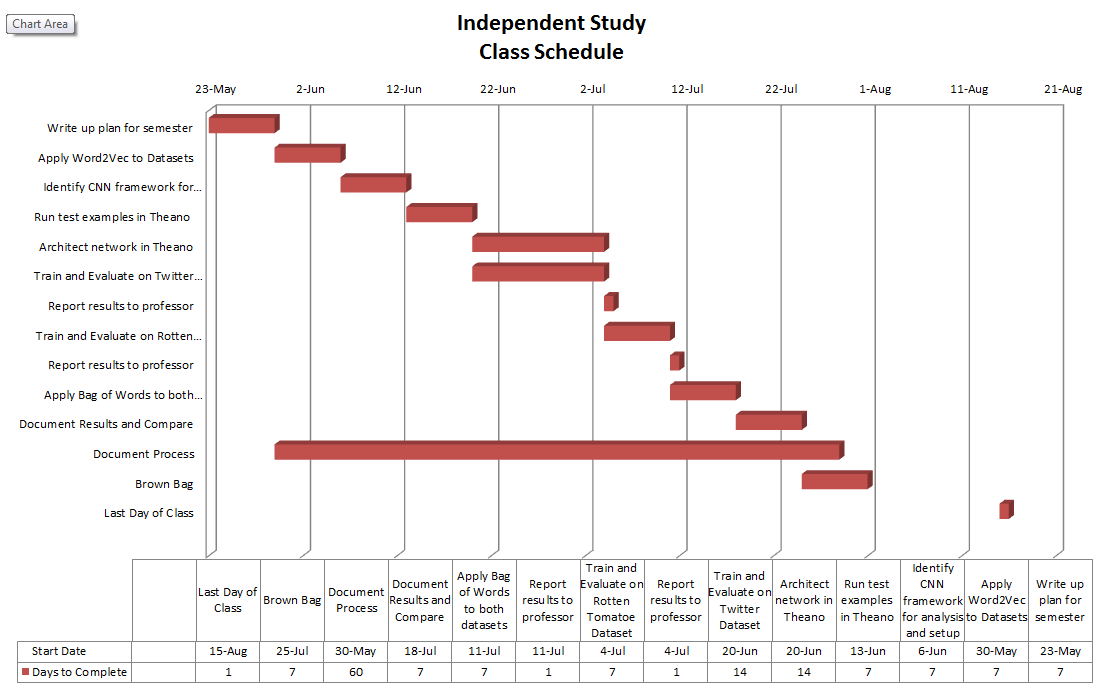
\includegraphics[scale=.5]{gantt.PNG}
  \caption{Project Development Schedule}
  \label{fig:schedule}
\end{figure}


\section{Co-occurence Matrices}

One of the more successful ideas from \ac{nlp} is the idea of using the surrounding words in a sentence to represent a word. This brought about the idea of the co-occurence matrix. This matrix captures the number of times a other word occurs directly next to it in a dataset. For example in the Standford Deep Learning Course \cite{dl_course}, they show the following example:

\begin{itemize}
	\item I like deep learning.
	\item I like NLP.
	\item I enjoy flying.
\end{itemize}

\begin{figure}[htbp!]
	\centering
	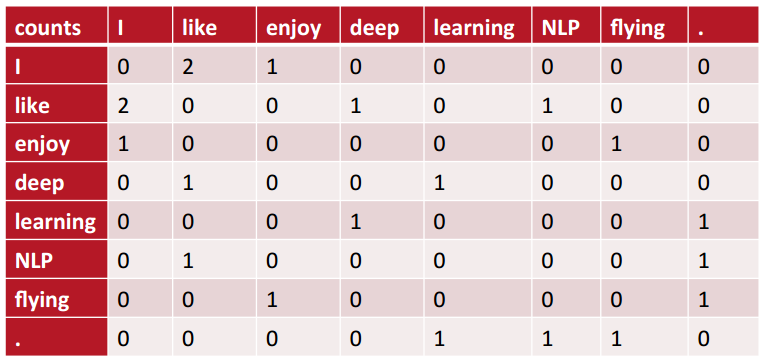
\includegraphics[scale=.4]{cooccurence.png}
	\caption{Co-occurence Matrix example.}
	\label{fig:cooccurence}
\end{figure}

This matrix shown in Figure \ref{fig:cooccurence} displays the number of times words appear next to each other in the three sentences above. The idea is that each row represents a feature vector that characterizes each word in the whole dataset.

There are obvious drawbacks to representing words in this way. One being that as the number of words in the dataset increases, so does the dimensionality of the matrix and as a result the vectors.

\section{Word2Vec}

This is a new technique \cite{word2vec} for predicting the words around a word and encoding this in a vector for classification.

Does not have the issues of co-occurrence matrices in that they are fast and flexible in terms of adding new words/sentences.

\section {Keras}
Keras \cite{chollet2015keras} is one of the many nerual network frameworks/libraries available for deep learning. Keras is very modular and supports \ac{cnn}s, \ac{rnn}s, and standard neural networks. Keras technically is a python wrapper around the Theano and TensorFlow deep learning frameworks. I decided to use this tool to construct \ac{cnn}s due to it's flexibility and rapid prototyping capability. Changing the number of filters in a \ac{cnn}, size, and\slash or number of fully connected layers is very simple. 


\section{IMDB Movie Review Dataset}
Dataset came with training and testing sets already defined. In total for training there were 24722 labeled reviews, and for testing there were a similar number of 24723 reviews that are unfortunately unlabeled. This dataset was attained through a Kaggle Data Science Competition. The competition has since ended but the dataset is still available. Since the hosted data was for a competition, Kaggle only provided the labeled training set. For this reason, I had to split the data to make my own training and test sets. The data was split 80\slash20 for training and testing respectively.

pos train: 9873
neg train: 9905

neg test = 2444
pos test = 2500

train 18000, 2000 validation, 5000 test
Vocabulary size = 81322 words

accuracy:86.06 percent

Confusion Matrices
[[1897  581]
[ 116 2406]]

[[ 0.77  0.23]
[ 0.05  0.95]]





\section{Twitter Sentiment Dataset}

Twitter is a social networking website \cite{twitter} where users can post 140 character messages on their accounts. Once the message is posted it is completely open to the entire Twitter user base. Twitter has evolved as a means of rapidly sharing information and events. For example, a company may choose to post that a new product is available on Twitter in addition to their website to reach a larger user base. Twitter posts are rich with sentiment and make it a good source for sentiment analysis.

To date there are no large hand labeled twitter datasets available for sentiment analysis. This led several Stanford Researchers \cite{Go_Bhayani_Huang_2009} to collect and build their own dataset called Sentiment140 \cite{sentiment140}. Labeling individual tweets for sentiment is a very tedious task, so the authors came up with a very creative way to mine positive and negative tweets. Twitter data was collected through the Twitter \ac{api} and labeled by using positive and negative emoticons. For example, if a tweet included a smiley face ":)" it was considered positive. If a tweet contained both a positive and negative emoticons the tweet was not used. The dataset was collected between April 6, 2009 to June 25, 2009.

In total there are 1.6 million tweets used for training. The number of positive and negative tweets are equal for train. The testing data is much smaller only containing 500 tweets. The tweets used for testing were hand labeled, where as the training tweets were mined.

Vocabulary Size 564692 words.
Max Sequence length was 52 words.

Based on paper Twitter Sentiment Classification using Distant Supervision \cite{Go_Bhayani_Huang_2009}. The dataset that they provide was

after 7 epochs
rand - 78 %
cnn-non-static - 75 % 75.98 %
cnn- static

\newpage
\bibliography{Austin_Dress_NLP_CNN_Summer_2016.bib}
\bibliographystyle{plain}




\end{document}
